\chapter{Orbitais atômicos: formas, energias e tamanhos}\label{ch:b2:atomic-orbitals}

Um átomo de hidrogênio não tem borda: seu elétron pode ser encontrado a
qualquer distância do núcleo, com uma probabilidade que diminui depressa, mas
nunca chega a zero. No entanto, os átomos têm tamanhos, e um átomo de sódio
é cerca de duas vezes mais largo que um átomo de cloro, embora tenha menos
elétrons. O volume do 1.º ano designou os estados de um elétron por três
números quânticos; aqui, cada um deles se torna uma função da posição, com
uma forma, nós, sinais e um tamanho, e um conjunto simples de regras os
transforma em \omterm{def:b2:atomic-orbitals:orbital-energy}{energias orbitais} para qualquer átomo. Essas formas e esses
sinais são o que os quatro capítulos seguintes combinam em orbitais
moleculares.

\begin{recall}
O volume do 1.º ano: os números quânticos $n$, $l$, $m_l$, $m_s$; os orbitais
atômicos como os estados $(n, l, m_l)$; camadas e subcamadas; blindagem e
carga nuclear efetiva (qualitativamente); configurações eletrônicas; os níveis
do hidrogênio, $-E_R/n^2$ com $E_R = \qty{13.6}{eV}$. Da física: a \omterm{def:b2:atomic-orbitals:wavefunction}{função de
onda}, cujo módulo ao quadrado é uma \omterm{def:b2:atomic-orbitals:wavefunction}{densidade de probabilidade}.
\end{recall}

\section{As funções de onda do átomo de hidrogênio}

\begin{definition}[Função de onda]\label{def:b2:atomic-orbitals:wavefunction}
O estado de um elétron é descrito por uma \emph{função de onda}\index{funcao de onda@função de onda}
$\psi(x, y, z)$; $|\psi|^2$ é sua \emph{densidade de probabilidade}\index{densidade de probabilidade}:
a probabilidade de encontrar o elétron em um pequeno volume $dV$ em torno de
um ponto é $|\psi|^2\,dV$, e $\int|\psi|^2\,dV = 1$ em todo o espaço (a função
está normalizada). Um orbital atômico é a função de onda de um elétron em um
átomo.
\end{definition}

\begin{definition}[Partes radial e angular]\label{def:b2:atomic-orbitals:radial-angular}
Em coordenadas esféricas $(r, \theta, \varphi)$ centradas no núcleo, os orbitais
de um átomo hidrogenoide se fatoram como $\psi_{nlm}(r, \theta, \varphi) = R_{nl}(r)\,
Y_{lm}(\theta, \varphi)$: a \emph{parte radial}\index{parte radial} $R_{nl}$ depende
de $n$ e $l$, a \emph{parte angular}\index{parte angular} $Y_{lm}$ apenas de $l$ e de
$m_l$.
\end{definition}

\begin{theorem}[Os orbitais hidrogenoides]\label{thm:b2:atomic-orbitals:hydrogen}
Para um átomo monoeletrônico de carga nuclear $Ze$, com $\rho = Zr/a_0$ e $a_0 =
\qty{52.9}{pm}$ o raio de Bohr, as \omterm{def:b2:atomic-orbitals:radial-angular}{partes radiais} para $n \leq 3$ são, em unidades de
$(Z/a_0)^{3/2}$:
\[
\begin{array}{ll}
  R_{1s} = 2\,\mathrm e^{-\rho} &
  R_{2s} = \dfrac{1}{2\sqrt2}\,(2 - \rho)\,\mathrm e^{-\rho/2} \\[2ex]
  R_{2p} = \dfrac{1}{2\sqrt6}\,\rho\,\mathrm e^{-\rho/2} &
  R_{3s} = \dfrac{2}{81\sqrt3}\,(27 - 18\rho + 2\rho^2)\,\mathrm e^{-\rho/3} \\[2ex]
  R_{3p} = \dfrac{4}{81\sqrt6}\,(6\rho - \rho^2)\,\mathrm e^{-\rho/3} &
  R_{3d} = \dfrac{4}{81\sqrt{30}}\,\rho^2\,\mathrm e^{-\rho/3}
\end{array}
\]
e as \omterm{def:b2:atomic-orbitals:radial-angular}{partes angulares} reais são $Y_s = 1/\sqrt{4\pi}$; $Y_{p_x}, Y_{p_y}, Y_{p_z} =
\sqrt{3/(4\pi)}\,(x, y, z)/r$; $Y_{d_{xy}} = \sqrt{15/(4\pi)}\,xy/r^2$ (e o mesmo para
$xz$, $yz$), $Y_{d_{x^2-y^2}} = \sqrt{15/(16\pi)}\,(x^2 - y^2)/r^2$, $Y_{d_{z^2}} =
\sqrt{5/(16\pi)}\,(3z^2 - r^2)/r^2$. Suas energias são $E_n = -Z^2E_R/n^2$.
% ledger: const:a0, const:RyhcEV
\end{theorem}

\admitted

Essas funções são as soluções da equação de Schrödinger para um elétron e um
núcleo, obtidas no volume do 3.º ano. As funções $p$ e $d$ reais são
combinações das complexas, rotuladas por $m_l$; elas apontam ao longo dos
eixos e são as usadas para construir ligações.

\begin{omfigure}
\begin{minipage}[t]{0.27\linewidth}\vspace{0pt}
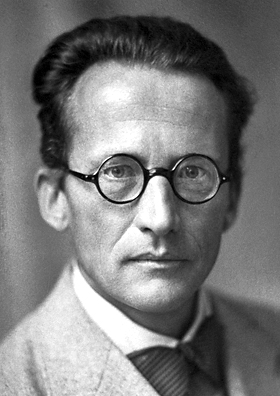
\includegraphics[width=\linewidth]{images/book3/schrodinger.jpg}
\end{minipage}\hfill
\begin{minipage}[t]{0.69\linewidth}\vspace{0pt}
{\small Erwin Schrödinger, que em 1926 escreveu a equação de onda cujas
soluções para o átomo de hidrogênio são os orbitais deste capítulo, e delas
recuperou os níveis de energia que Bohr havia postulado. Dividiu o Prêmio
Nobel de Física de 1933. (Fotografia: Fundação Nobel, domínio público,
Wikimedia Commons.)}
\end{minipage}
\end{omfigure}

\section{A parte radial}

A probabilidade de encontrar o elétron entre as esferas de raios $r$ e $r +
dr$ é $|\psi|^2$ integrado sobre a casca de volume $4\pi r^2\,dr$; para qualquer
orbital, uma vez integrados os ângulos, ela vale $r^2R^2\,dr$.

\begin{definition}[Distribuição radial]\label{def:b2:atomic-orbitals:radial-distribution}
A \emph{função de distribuição radial}\index{funcao de distribuicao radial@função de distribuição radial} de
um orbital é $P(r) = r^2R_{nl}(r)^2$: $P(r)\,dr$ é a probabilidade de o
elétron estar entre $r$ e $r + dr$ do núcleo. O \emph{raio mais
provável}\index{raio mais provavel@raio mais provável} é o valor de $r$ em seu maior máximo.
\end{definition}

\begin{proposition}[Normalização do 1s]\label{prop:b2:atomic-orbitals:normalised}
$\int_0^\infty P_{1s}(r)\,dr = 1$.
\end{proposition}

\begin{proof}
Com $Z = 1$ e $r$ em unidades de $a_0$, $P_{1s} = 4r^2\mathrm e^{-2r}$. Integrando por partes duas vezes,
$\int_0^\infty r^2\mathrm e^{-2r}\,dr = \frac22\int_0^\infty r\,\mathrm e^{-2r}\,dr =
\frac12\int_0^\infty\mathrm e^{-2r}\,dr = \frac14$, and $4 \times \frac14 = 1$.
\end{proof}

\begin{proposition}[Raio mais provável]\label{prop:b2:atomic-orbitals:most-probable}
Para o orbital 1s, o \omterm{def:b2:atomic-orbitals:radial-distribution}{raio mais provável} é $a_0/Z$. Para um orbital com $l =
n - 1$ (1s, 2p, 3d, \dots), ele vale $n^2a_0/Z$.
\end{proposition}

\begin{proof}
Para $l = n - 1$, a \omterm{def:b2:atomic-orbitals:radial-angular}{parte radial} não tem nó: $R \propto \rho^{n-1}\mathrm e^{-\rho/n}$,
logo $P \propto \rho^{2n}\mathrm e^{-2\rho/n}$ e $d\ln P/d\rho = 2n/\rho - 2/n$, nula
para $\rho = n^2$, isto é, $r = n^2a_0/Z$. Com $n = 1$, $r = a_0/Z$.
\end{proof}

\begin{proposition}[Raio médio do 1s]\label{prop:b2:atomic-orbitals:mean-radius}
A distância média de um elétron 1s ao núcleo é $\langle r\rangle = 3a_0/(2Z)$,
maior que seu \omterm{def:b2:atomic-orbitals:radial-distribution}{raio mais provável}.
\end{proposition}

\begin{proof}
Com $Z = 1$: $\langle r\rangle = \int_0^\infty r\,P(r)\,dr = 4\int_0^\infty r^3\mathrm e^{-2r}
\,dr = 4 \times 3!/2^4 = 3/2$. A distribuição tem uma longa cauda para $r$
grande, que puxa a média para além do máximo.
\end{proof}

\begin{definition}[Nós]\label{def:b2:atomic-orbitals:node}
Uma \emph{superfície nodal}\index{superficie nodal@superfície nodal} de um orbital é uma superfície na
qual a \omterm{def:b2:atomic-orbitals:wavefunction}{função de onda} se anula e muda de sinal. É um \emph{nó radial}\index{no radial@nó radial}
(uma esfera) quando a \omterm{def:b2:atomic-orbitals:radial-angular}{parte radial} se anula, e um \emph{nó
angular}\index{no angular@nó angular} (um plano ou um cone que passa pelo núcleo) quando a
\omterm{def:b2:atomic-orbitals:radial-angular}{parte angular} se anula.
\end{definition}

\begin{proposition}[Contagem dos nós]\label{prop:b2:atomic-orbitals:nodes}
Um orbital $(n, l)$ tem $n - l - 1$ \omterm{def:b2:atomic-orbitals:node}{nós radiais} e $l$ \omterm{def:b2:atomic-orbitals:node}{nós angulares}, $n - 1$
ao todo.
\end{proposition}

\begin{proof}
Nas funções do \cref{thm:b2:atomic-orbitals:hydrogen}: $R_{2s}$ se anula em
$\rho = 2$, $R_{3s}$ nas duas raízes de $2\rho^2 - 18\rho + 27$ ($\rho = 1.90$ e $7.10$),
$R_{3p}$ em $\rho = 6$; $R_{1s}$, $R_{2p}$, $R_{3d}$ não se anulam. A \omterm{def:b2:atomic-orbitals:radial-angular}{parte angular}
de um orbital p se anula em um plano ($z = 0$ para $p_z$), a de um orbital d em
dois planos ou, para $d_{z^2}$, em um cone. O caso geral é admitido.
\end{proof}

\begin{omfigure}
\begin{tikzpicture}
\begin{axis}[width=0.55\linewidth, height=6cm, xmin=0, xmax=24, ymin=0, ymax=0.58,
  axis x line=bottom, axis y line=left, xlabel={$r/a_0$}, ylabel={$P(r)$},
  tick label style={font=\small}, label style={font=\small}, title={\small distribuições radiais, $Z = 1$}]
\addplot[omThm, thick] table[x=r, y=s1] {figdata/out/bachelor-2-atomic-orbitals-a.dat};
\addplot[omDef, thick] table[x=r, y=s2] {figdata/out/bachelor-2-atomic-orbitals-a.dat};
\addplot[omDef, thick, dashed] table[x=r, y=p2] {figdata/out/bachelor-2-atomic-orbitals-a.dat};
\addplot[omProp, thick] table[x=r, y=s3] {figdata/out/bachelor-2-atomic-orbitals-a.dat};
\addplot[omProp, thick, dashed] table[x=r, y=p3] {figdata/out/bachelor-2-atomic-orbitals-a.dat};
\addplot[omProp, thick, dotted] table[x=r, y=d3] {figdata/out/bachelor-2-atomic-orbitals-a.dat};
\node[font=\scriptsize, omThm, anchor=west] at (axis cs:1.4,0.53) {1s};
\node[font=\scriptsize, omDef, anchor=south] at (axis cs:4.0,0.215) {2p};
\node[font=\scriptsize, omDef, anchor=south west] at (axis cs:6.4,0.17) {2s};
\node[font=\scriptsize, omProp, anchor=south] at (axis cs:10.5,0.12) {3d};
\node[font=\scriptsize, omProp, anchor=west] at (axis cs:17,0.085) {3s, 3p};
\end{axis}
\end{tikzpicture}\hfill
\begin{tikzpicture}
\begin{axis}[width=0.42\linewidth, height=6cm, xmin=0, xmax=20, ymin=-0.12, ymax=0.75,
  axis x line=middle, axis y line=left, xlabel={$r/a_0$}, ylabel={$R$},
  tick label style={font=\small}, label style={font=\small}, title={\small partes radiais}]
\addplot[omDef, thick] table[x=r, y=R2s] {figdata/out/bachelor-2-atomic-orbitals-b.dat};
\addplot[omProp, thick] table[x=r, y=R3s] {figdata/out/bachelor-2-atomic-orbitals-b.dat};
\node[font=\scriptsize, omDef, anchor=west] at (axis cs:0.4,0.62) {$R_{2s}$};
\node[font=\scriptsize, omProp, anchor=west] at (axis cs:0.6,0.30) {$R_{3s}$};
\node[font=\scriptsize, anchor=south west] at (axis cs:3,0.15) {nó};
\draw[thin, ->] (axis cs:3,0.15) -- (axis cs:2.05,0.01);
\end{axis}
\end{tikzpicture}

{\small À esquerda: distribuições radiais $P(r) = r^2R^2$ dos orbitais do
hidrogênio até $n = 3$; quanto maior $n$, mais longe o elétron, e os orbitais s
têm pequenos máximos internos (penetração). À direita: $R_{2s}$ e $R_{3s}$ mudam
de sinal em seus \omterm{def:b2:atomic-orbitals:node}{nós radiais} ($r = 2a_0$; $1.90a_0$ e $7.10a_0$).}
\end{omfigure}

\begin{omfigure}
\begin{tikzpicture}
\begin{axis}[scale only axis, width=0.32\linewidth, height=0.32\linewidth,
  xmin=-6, xmax=6, ymin=-6, ymax=6, axis lines=none, title={\small 1s}]
\addplot[only marks, mark=*, mark size=0.25pt, omDef] table[x=x, y=y] {figdata/out/bachelor-2-atomic-orbitals-c-1s.dat};
\end{axis}
\end{tikzpicture}\hspace{0.12\linewidth}%
\begin{tikzpicture}
\begin{axis}[scale only axis, width=0.32\linewidth, height=0.32\linewidth,
  xmin=-14, xmax=14, ymin=-14, ymax=14, axis lines=none, title={\small 2s}]
\addplot[only marks, mark=*, mark size=0.25pt, omDef] table[x=x, y=y] {figdata/out/bachelor-2-atomic-orbitals-c-2s.dat};
\draw[densely dashed, omThm] (axis cs:0,0) circle[radius=2];
\end{axis}
\end{tikzpicture}

{\small Representações por densidade de pontos dos orbitais 1s e 2s do
hidrogênio em um plano que passa pelo núcleo: a densidade de pontos segue
$|\psi|^2$ (amostragem determinística). A nuvem 2s tem um anel vazio, o \omterm{def:b2:atomic-orbitals:node}{nó
radial} em $2a_0$ (tracejado); os quadros têm 12 e 28 $a_0$ de largura.}
\end{omfigure}

\section{A parte angular}

A \omterm{def:b2:atomic-orbitals:radial-angular}{parte angular} fixa a forma. Um orbital s é esférico; um orbital p tem dois
lobos de sinais opostos ao longo de seu eixo, separados por um plano nodal; um
orbital d tem quatro lobos de sinais alternados (ou, para $d_{z^2}$, dois lobos
e um anel). O sinal de um lobo não tem significado físico por si só --- $\psi$
e $-\psi$ descrevem o mesmo estado ---, mas os sinais relativos de dois
orbitais decidem, no próximo capítulo, se eles se combinam em uma ligação.

\begin{omfigure}
\begin{tikzpicture}[font=\small]
  \pic at (0,0) {oms={1}};
  \node[below] at (0,-0.75) {s};
  \pic at (2.0,0) {omp={1}{0}};
  \draw[->, black!55, thin] (1.0,0) -- (3.0,0) node[right, font=\tiny] {$x$};
  \node[below] at (2.0,-0.75) {$\mathrm p_x$};
  \pic at (4.2,0) {omp={1}{90}};
  \draw[->, black!55, thin] (4.2,-0.95) -- (4.2,0.95) node[above, font=\tiny] {$z$};
  \node[below] at (4.75,-0.75) {$\mathrm p_z$};
  \pic at (6.6,0) {omdxy}; \node[below] at (6.6,-1.0) {$\mathrm d_{xy}$};
  \pic at (9.0,0) {omdx2y2}; \node[below] at (9.0,-1.0) {$\mathrm d_{x^2-y^2}$};
  \pic at (11.4,0) {omdz2}; \node[below] at (11.4,-1.0) {$\mathrm d_{z^2}$};
\end{tikzpicture}

{\small Orbitais atômicos reais, esquemáticos: os lobos mostram as regiões em
que $|\psi|$ é grande, coloridas pelo sinal de $\psi$ (azul positivo, laranja
negativo). Os orbitais $\mathrm d_{xz}$ e $\mathrm d_{yz}$ têm a forma de
$\mathrm d_{xy}$ nos planos que seus nomes indicam.}
\end{omfigure}

\begin{method}[Esboçar um orbital a partir de seus números quânticos]\label{met:b2:atomic-orbitals:draw-orbital}
\begin{enumerate}
  \item A partir de $l$, a forma: s (esfera), p (dois lobos), d (quatro lobos,
        ou dois lobos e um anel para $d_{z^2}$); a partir do índice, a orientação.
  \item Conte os $l$ \omterm{def:b2:atomic-orbitals:node}{nós angulares} (planos que passam pelo núcleo) e dê sinais
        opostos aos lobos adjacentes.
  \item Conte os $n - l - 1$ \omterm{def:b2:atomic-orbitals:node}{nós radiais}: camadas internas de sinal oposto
        dentro dos lobos principais (em geral omitidas nos esboços).
  \item Ajuste a escala com $n^2a_0/Z$: $n$ maior, orbital maior; $Z$ maior,
        orbital menor.
\end{enumerate}
\end{method}

\section{Átomos polieletrônicos}

Em um átomo com vários elétrons, cada elétron sente o núcleo blindado pelos
outros. Os orbitais conservam as formas dos do hidrogênio, com uma carga
efetiva $Z^*$ no lugar de $Z$, e a energia de uma subcamada passa a depender de
$l$ além de $n$: um elétron s, cuja distribuição radial tem máximos internos
perto do núcleo, é menos blindado que um elétron p da mesma camada, e um p
menos que um d.

\begin{definition}[Regras de Slater]\label{def:b2:atomic-orbitals:slater}
As \emph{regras de Slater}\index{regras de Slater} estimam a carga nuclear efetiva
$Z^* = Z - \sigma$ sentida por um elétron. Os elétrons são agrupados como
(1s) (2s, 2p) (3s, 3p) (3d) (4s, 4p) (4d) (4f) (5s, 5p) \dots; a constante de
blindagem $\sigma$ de um elétron é a soma das contribuições dos outros
elétrons: 0.35 para cada outro elétron do mesmo grupo (0.30 dentro do 1s);
para um elétron s ou p, 0.85 para cada elétron da camada $n - 1$ e 1.00 para
cada elétron das camadas inferiores; para um elétron d ou f, 1.00 para todo
elétron dos grupos abaixo do seu. Os grupos acima não contribuem.
\end{definition}

\begin{omfigure}
\small
\renewcommand{\arraystretch}{1.2}
\begin{tabular}{l|ccccc}
elétron estudado & mesmo grupo & camada $n - 1$ & camadas inferiores & grupos acima \\ \hline
1s & 0.30 & --- & --- & 0 \\
$n$s, $n$p & 0.35 & 0.85 & 1.00 & 0 \\
$n$d, $n$f & 0.35 & 1.00 & 1.00 & 0 \\
\end{tabular}

\smallskip
{\small Constantes de blindagem de Slater, por elétron blindante. Os números
quânticos principais efetivos são $n^* = 1, 2, 3, 3.7, 4.0, 4.2$ para $n = 1$ a 6.}
\end{omfigure}

\begin{method}[Calcular uma carga efetiva]\label{met:b2:atomic-orbitals:slater}
\begin{enumerate}
  \item Escreva a configuração nos grupos de Slater, em ordem de $n$, com s e p
        juntos e d e f à parte.
  \item Escolha o elétron; some 0.35 para cada outro elétron de seu grupo.
  \item Some 0.85 (elétron s ou p) ou 1.00 (d ou f) por elétron da camada
        logo abaixo, e 1.00 por elétron mais profundo.
  \item $Z^* = Z - \sigma$.
\end{enumerate}
\end{method}

\begin{definition}[Energia e raio orbitais]\label{def:b2:atomic-orbitals:orbital-energy}
No modelo de Slater, a \emph{energia orbital}\index{energia orbital} de um elétron
de carga efetiva $Z^*$ e número quântico principal efetivo $n^*$ é
$\varepsilon = -E_RZ^{*2}/n^{*2}$, e seu \emph{raio orbital}\index{raio orbital}
é $n^{*2}a_0/Z^*$, o \omterm{def:b2:atomic-orbitals:radial-distribution}{raio mais provável} de um orbital hidrogenoide de carga
$Z^*$.
\end{definition}

\begin{proposition}[Energias de Slater]\label{prop:b2:atomic-orbitals:slater-energy}
A energia de um grupo de $k$ elétrons de carga efetiva $Z^*$ é aproximadamente
$k\varepsilon = -kE_RZ^{*2}/n^{*2}$, e a energia eletrônica total do átomo é a
soma sobre seus grupos.
\end{proposition}

\admitted

\begin{example}[Ferro: 4s ou 3d primeiro?]\label{ex:b2:atomic-orbitals:iron}
O ferro é $[\ce{Ar}]\,3\mathrm d^6\,4\mathrm s^2$. Um elétron 4s: $\sigma = 0.35 + 14
\times 0.85 + 10 \times 1.00 = 22.25$, $Z^* = 3.75$, $\varepsilon = -13.6 \times
3.75^2/3.7^2 = \qty{-14.0}{eV}$. Um elétron 3d: $\sigma = 5 \times 0.35 + 18 \times 1.00 =
19.75$, $Z^* = 6.25$, $\varepsilon = -13.6 \times 6.25^2/9 = \qty{-59}{eV}$. Os
elétrons 3d estão muito mais fortemente ligados: embora o 4s seja preenchido
primeiro na ordem de preenchimento, é um elétron 4s que sai quando o ferro é
ionizado, e o íon ferro(II) é $[\ce{Ar}]\,3\mathrm d^6$.
\end{example}

\section{Usar as energias e os tamanhos orbitais}

\begin{proposition}[Energia de ionização a partir das energias de Slater]\label{prop:b2:atomic-orbitals:ionisation}
No modelo de Slater, a primeira energia de ionização de um átomo é a diferença
entre as energias totais do íon e do átomo, calculadas grupo a grupo com as
cargas efetivas de cada um.
\end{proposition}

\begin{proof}
A energia de ionização é $E(\text{íon}) - E(\text{átomo})$; pela
\cref{prop:b2:atomic-orbitals:slater-energy}, ambas são somas de energias de
grupo, e só muda o grupo que perde o elétron (os grupos internos não são
blindados pelos elétrons externos).
\end{proof}

\begin{example}[O carbono]\label{ex:b2:atomic-orbitals:carbon}
Carbono, (2s, 2p)$^4$: $Z^* = 6 - 2 \times 0.85 - 3 \times 0.35 = 3.25$; a energia do grupo é
$4 \times (-13.6 \times 3.25^2/4) = \qty{-143.6}{eV}$. O íon \ce{C+}, (2s, 2p)$^3$: $Z^* =
3.60$, $3 \times (-13.6 \times 3.60^2/4) = \qty{-132.2}{eV}$. A energia de ionização é
\qty{11.5}{eV}, contra \qty{11.26}{eV} medidos.
% ledger: ie:C, const:RyhcEV
\end{example}

\begin{omfigure}
\begin{tikzpicture}
\begin{axis}[width=0.47\linewidth, height=5.4cm, xmin=0.5, xmax=8.5, ymin=0, ymax=6.5,
  axis x line=bottom, axis y line=left, xtick={1,2,3,4,5,6,7,8},
  xticklabels={Li,Be,B,C,N,O,F,Ne}, tick label style={font=\small},
  label style={font=\small}, title={\small período 2}]
\addplot[omThm, thick, mark=*, mark size=1.3pt] table[x=k, y=zs] {figdata/out/bachelor-2-atomic-orbitals-d-period.dat};
\addplot[omDef, thick, mark=square*, mark size=1.3pt] table[x=k, y=r] {figdata/out/bachelor-2-atomic-orbitals-d-period.dat};
\node[font=\scriptsize, omThm, anchor=south east] at (axis cs:7.8,5.3) {$Z^*$};
\node[font=\scriptsize, omDef, anchor=south west] at (axis cs:1.2,3.1) {raio ($a_0$)};
\end{axis}
\end{tikzpicture}\hfill
\begin{tikzpicture}
\begin{axis}[width=0.47\linewidth, height=5.4cm, xmin=1.5, xmax=6.5, ymin=0, ymax=9,
  axis x line=bottom, axis y line=left, xtick={2,3,4,5,6},
  xticklabels={Li,Na,K,Rb,Cs}, tick label style={font=\small},
  label style={font=\small}, title={\small grupo 1}]
\addplot[omThm, thick, mark=*, mark size=1.3pt] table[x=n, y=zs] {figdata/out/bachelor-2-atomic-orbitals-d-group.dat};
\addplot[omDef, thick, mark=square*, mark size=1.3pt] table[x=n, y=r] {figdata/out/bachelor-2-atomic-orbitals-d-group.dat};
\node[font=\scriptsize, omThm, anchor=north] at (axis cs:4,2.0) {$Z^*$};
\node[font=\scriptsize, omDef, anchor=west] at (axis cs:2.1,5.4) {raio ($a_0$)};
\end{axis}
\end{tikzpicture}

{\small Carga efetiva de Slater do elétron de valência e \omterm{def:b2:atomic-orbitals:orbital-energy}{raio orbital}
$n^{*2}a_0/Z^*$. Ao longo do período 2, $Z^*$ cresce 0.65 por elemento e os
átomos encolhem; descendo o grupo 1, $Z^*$ fica em 1.30 e depois 2.20 enquanto
$n^*$ cresce, e os átomos incham.}
\end{omfigure}

O modelo reproduz as tendências do volume do 1.º ano. Ao longo de um período,
cada próton acrescentado é blindado por apenas 0.35 do elétron acrescentado com
ele: $Z^*$ sobe, o orbital externo se contrai e liga mais fortemente. Descendo
um grupo, $Z^*$ quase não muda enquanto a camada externa se afasta: os átomos
crescem e suas energias de ionização caem. O sódio, com $Z^* = 2.20$ para seu
elétron 3s, tem um \omterm{def:b2:atomic-orbitals:orbital-energy}{raio orbital} de $9/2.2 = 4.1a_0$; o cloro, com $Z^* = 6.10$
para um elétron 3p, $9/6.1 = 1.5a_0$.

\section{Exercícios}

\begin{exercise}[$\star$]\label{exo:b2:atomic-orbitals:1}
Dê os números quânticos $n$ e $l$, o número de \omterm{def:b2:atomic-orbitals:node}{nós radiais} e de \omterm{def:b2:atomic-orbitals:node}{nós angulares}
de um orbital 3p e de um orbital 4d.
\end{exercise}

\begin{exercise}[$\star$]\label{exo:b2:atomic-orbitals:2}
Mostre, a partir de $R_{2p}$, que o \omterm{def:b2:atomic-orbitals:radial-distribution}{raio mais provável} de um elétron 2p do
hidrogênio é $4a_0$, e dê-o em picômetros.
\end{exercise}

\begin{exercise}[$\star$]\label{exo:b2:atomic-orbitals:3}
Calcule a probabilidade de encontrar o elétron 1s do hidrogênio mais perto do
núcleo do que $a_0$.
\end{exercise}

\begin{exercise}[$\star$]\label{exo:b2:atomic-orbitals:4}
Esboce o orbital $3\mathrm d_{xy}$: lobos, sinais, planos nodais. Quantos \omterm{def:b2:atomic-orbitals:node}{nós
radiais} ele tem?
\end{exercise}

\begin{exercise}[$\star\star$]\label{exo:b2:atomic-orbitals:5}
Calcule a carga efetiva de Slater de um elétron 2p do oxigênio e o \omterm{def:b2:atomic-orbitals:orbital-energy}{raio
orbital} que ela dá.
\end{exercise}

\begin{exercise}[$\star\star$]\label{exo:b2:atomic-orbitals:6}
Usando o exemplo do ferro, explique por que a configuração de \ce{Fe^3+} é
$[\ce{Ar}]\,3\mathrm d^5$ e não $[\ce{Ar}]\,3\mathrm d^3 4\mathrm s^2$.
\end{exercise}

\begin{exercise}[$\star\star$]\label{exo:b2:atomic-orbitals:7}
Estime pelas \omterm{def:b2:atomic-orbitals:slater}{regras de Slater} as primeiras energias de ionização do lítio e do
sódio e compare com os valores medidos, 5.39 e \qty{5.14}{eV}. Comente.
\end{exercise}

\begin{exercise}[$\star\star$]\label{exo:b2:atomic-orbitals:8}
Calcule $Z^*$ e o \omterm{def:b2:atomic-orbitals:orbital-energy}{raio orbital} do elétron externo do sódio e do cloro, e
explique por que o átomo de sódio é o maior.
\end{exercise}

\begin{exercise}[$\star\star$]\label{exo:b2:atomic-orbitals:9}
Mostre que os orbitais 1s e 2s do hidrogênio são ortogonais,
$\int\psi_{1s}\psi_{2s}\,dV = 0$.
\end{exercise}

\begin{exercise}[$\star\star\star$]\label{exo:b2:atomic-orbitals:10}
Escreva $R_{2p} = N\rho\,\mathrm e^{-\rho/2}$ e encontre a constante $N$ que a normaliza
($Z = 1$, $r$ em unidades de $a_0$).
\end{exercise}

\begin{exercise}[$\star\star\star$]\label{exo:b2:atomic-orbitals:11}
Compare o raio médio e o \omterm{def:b2:atomic-orbitals:radial-distribution}{raio mais provável} de um elétron 1s e explique, a
partir da forma de $P(r)$, por que eles diferem.
\end{exercise}

\begin{exercise}[$\star\star\star$]\label{exo:b2:atomic-orbitals:12}
Encontre a \omterm{def:b2:atomic-orbitals:node}{superfície nodal} do orbital $\mathrm p_z$ e mostre que $\psi_{2p_z}$
muda de sinal através dela. Qual é a \omterm{def:b2:atomic-orbitals:wavefunction}{densidade de probabilidade} nessa superfície?
\end{exercise}

\section{Problema: Onde está o elétron?}

\begin{problem}[{Problema de fim de semana --- o orbital 1s do hidrogênio e seus
raios, a probabilidade de encontrar o elétron além de uma dada distância, os
nós e os máximos de 2s e 2p, e a estimativa de Slater das energias de
ionização do carbono, do nitrogênio e do oxigênio}]
\label{pb:b2:atomic-orbitals:1}
Dados: $a_0 = \qty{52.9}{pm}$; $E_R = \qty{13.6}{eV}$; primeiras energias de
ionização medidas (\unit{eV}): C 11.26, N 14.53, O 13.62. $\psi_{1s} = \pi^{-1/2}a_0^{-3/2}\,
\mathrm e^{-r/a_0}$.
% ledger: const:a0, const:RyhcEV, ie:C, ie:N, ie:O

\medskip
\noindent\textbf{Parte I --- O orbital 1s.}
\begin{enumerate}
  \item Verifique que $\psi_{1s}$ está normalizada, usando $dV = 4\pi r^2\,dr$.
  \item Escreva a \omterm{def:b2:atomic-orbitals:radial-distribution}{função de distribuição radial} $P(r)$.
  \item Encontre o \omterm{def:b2:atomic-orbitals:radial-distribution}{raio mais provável}.
  \item Calcule o raio médio.
  \item Por que a média é maior que o \omterm{def:b2:atomic-orbitals:radial-distribution}{raio mais provável}?
  \item A \omterm{def:b2:atomic-orbitals:wavefunction}{densidade de probabilidade} é máxima no núcleo, e no entanto $P(0) = 0$.
        Explique.
  \item Dê o \omterm{def:b2:atomic-orbitals:radial-distribution}{raio mais provável} em picômetros.
\end{enumerate}

\medskip
\noindent\textbf{Parte II --- Além de um raio.}
\begin{enumerate}[resume]
  \item Mostre que a probabilidade de encontrar o elétron além de $r_0 =
        xa_0$ é $\mathrm e^{-2x}(1 + 2x + 2x^2)$.
  \item Calcule-a para $r_0 = a_0$.
  \item Calcule-a para $r_0 = 2a_0$.
  \item Encontre por tentativas o raio da esfera que contém o elétron com uma
        probabilidade de 0.90.
  \item Em que sentido um átomo não tem borda, e em que sentido tem um tamanho?
\end{enumerate}

\medskip
\noindent\textbf{Parte III --- 2s e 2p.}
\begin{enumerate}[resume]
  \item Dê os nós de 2s e de 2p (número, tipo, posição).
  \item Onde $R_{2s}$ muda de sinal?
  \item Encontre o \omterm{def:b2:atomic-orbitals:radial-distribution}{raio mais provável} de 2p.
  \item Encontre os dois máximos de $P_{2s} \propto r^2(2 - r)^2\mathrm e^{-r}$ ($r$ em unidades de
        $a_0$).
  \item Qual de 2s e 2p tem densidade eletrônica mais perto do núcleo? O que
        isso implica em um átomo polieletrônico?
  \item Como esses raios mudam para o íon hidrogenoide \ce{C^5+}?
\end{enumerate}

\medskip
\noindent\textbf{Parte IV --- Carbono, nitrogênio, oxigênio.}
\begin{enumerate}[resume]
  \item Calcule o $Z^*$ de Slater de um elétron 2p em C, N e O.
  \item Calcule as \omterm{def:b2:atomic-orbitals:orbital-energy}{energias orbitais} correspondentes.
  \item Estime a primeira energia de ionização do carbono como diferença de
        energias de grupo.
  \item O mesmo para o nitrogênio.
  \item O mesmo para o oxigênio, e compare os três com os valores medidos.
  \item Que característica dos valores medidos o modelo não capta, e por quê?
  \item Dê a probabilidade de encontrar o elétron 1s do hidrogênio além de
        $2a_0$.
\end{enumerate}
\end{problem}
